% Generated 2020-01-10 13:32:54 -0800
\subsection{Components} \label{model:Components}

\begin{figure}[ht]
  \centering
    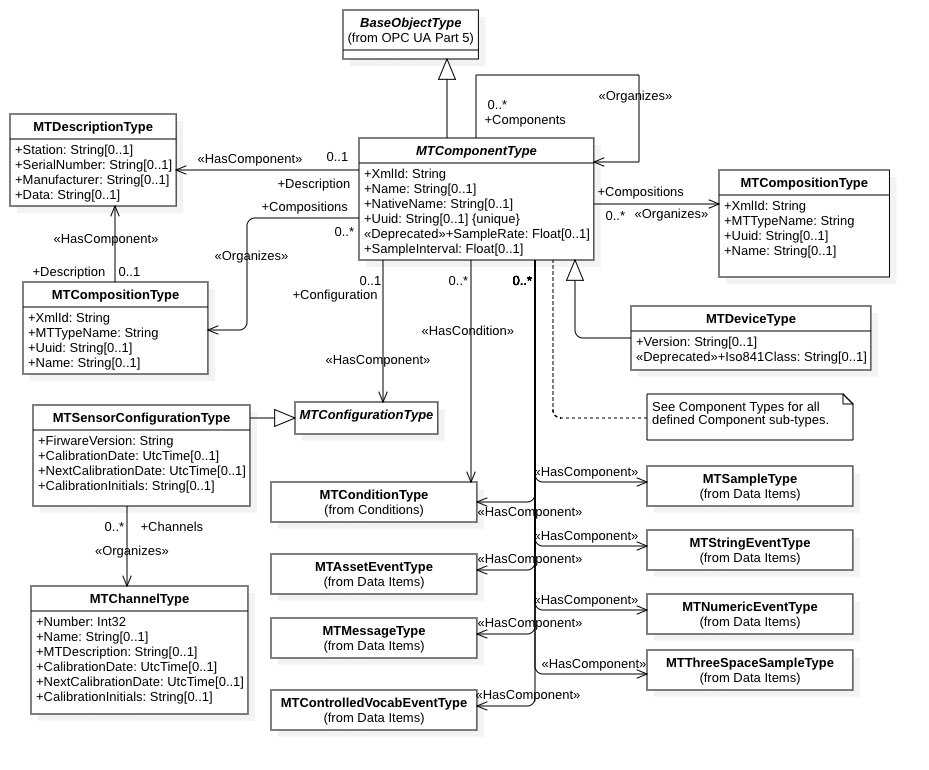
\includegraphics[width=1.0\textwidth]{./diagrams/types/Components.png}
  \caption{Components Diagram}
  \label{fig:Components}
\end{figure}

\FloatBarrier


The \glspl{MTComponent} documents the Component models and the owned objects.

\subsubsection{Defintion of \texttt{ MTChannelType}}
  \label{type:MTChannelType}

\FloatBarrier

A Channel of a sensor.

See ChannelType in type specifications.

channel represents each sensing element connected to a sensor unit.

\begin{table}[ht]
\centering 
  \caption{\texttt{MTChannelType} Definition}
  \label{table:MTChannelType}
\fontsize{9pt}{11pt}\selectfont
\tabulinesep=3pt
\begin{tabu} to 6in {|X[-1.35]|X[-0.7]|X[-1.75]|X[-1.5]|X[-1]|X[-0.7]|} \everyrow{\hline}
\hline
\rowfont\bfseries {Attribute} & \multicolumn{5}{|l|}{Value} \\
\tabucline[1.5pt]{}
BrowseName & \multicolumn{5}{|l|}{MTChannelType} \\
IsAbstract & \multicolumn{5}{|l|}{False} \\
\tabucline[1.5pt]{}
\rowfont \bfseries References & NodeClass & BrowseName & DataType & Type\-Definition & {Modeling\-Rule} \\
\multicolumn{6}{|l|}{Subtype of BaseObjectType (See \cite{UAPart5} Documentation)} \\
Has\-Property & Variable & Calibration\-Date & Utc\-Time & Property\-Type & Optional \\
Has\-Property & Variable & Calibration\-Initials & String & Property\-Type & Optional \\
Has\-Property & Variable & MT\-Description & String & Property\-Type & Optional \\
Has\-Property & Variable & Name & String & Property\-Type & Optional \\
Has\-Property & Variable & Next\-Calibration\-Date & Utc\-Time & Property\-Type & Optional \\
Has\-Property & Variable & Number & Int32 & Property\-Type & Mandatory \\
\end{tabu}
\end{table} 


\FloatBarrier
\paragraph{Referenced Properties and Objects}

\begin{itemize}
\item \texttt{CalibrationDate : UtcTime:}  Date upon which the sensor unit was last calibrated. 

\item \texttt{CalibrationInitials : String:}  The initials of the person verifying the validity of the calibration data.

\item \texttt{Name : String:}  The name of an element or a piece of equipment.

\item \texttt{NextCalibrationDate : UtcTime:}  Date upon which the sensor unit is next scheduled to be calibrated. 

\item \texttt{Number : Int32:}  A unique identifier that will only refer to a specific sensing element.

\end{itemize}
\FloatBarrier
\subsubsection{Defintion of \texttt{ MTComponentType}}
  \label{type:MTComponentType}

\FloatBarrier

\begin{figure}[ht]
  \centering
    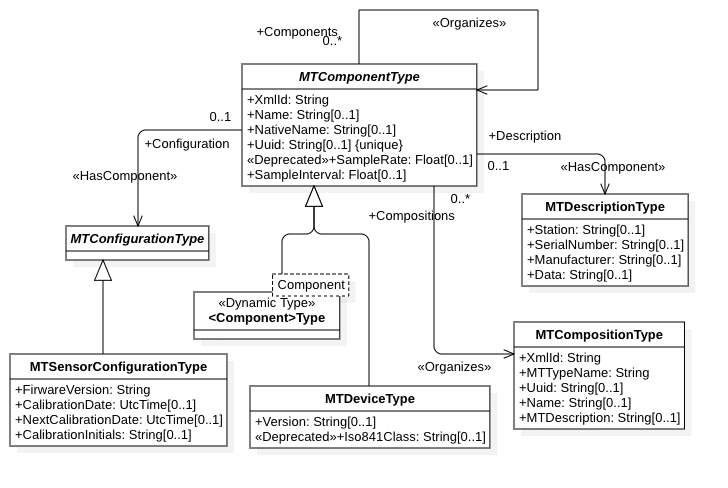
\includegraphics[width=1.0\textwidth]{./diagrams/types/MTComponentType.png}
  \caption{MTComponentType Diagram}
  \label{fig:MTComponentType}
\end{figure}

\FloatBarrier


The base \gls{MTComponent} Type from which all MTConnect Components are derived.
The component types will be created once for all \gls{MTComponent} \glspl{Object}
of that type based on the \gls{QName} of the MTConnect XML element. 

The Component Objects will be created and inserted into the \mtmodel{Components} 
folder with a \gls{BrowseName} of the Component \gls{QName} and the \mtmodel{name} element if specified surrounded 
by square brackets, \texttt{[]}. For example if the MTConnect Element is:

\xml{<Linear name='X'>...</...>}

The OPC UA Object with \gls{BrowseName} \xml{Linear[X]} will be created with the \uamodel{HasTypeDefinition}
referencing the \mtmodel{Linear} OPC UA \gls{Type}. 

The meta data for the component and its relationships are static. The dynamic data will be 
represented using the \cite{UAPart8}.

An abstract XML element. Replaced in the XML document by types of component elements representing physical parts and logical functions of a piece of equipment.

\begin{table}[ht]
\centering 
  \caption{\texttt{MTComponentType} Definition}
  \label{table:MTComponentType}
\fontsize{9pt}{11pt}\selectfont
\tabulinesep=3pt
\begin{tabu} to 6in {|X[-1.35]|X[-0.7]|X[-1.75]|X[-1.5]|X[-1]|X[-0.7]|} \everyrow{\hline}
\hline
\rowfont\bfseries {Attribute} & \multicolumn{5}{|l|}{Value} \\
\tabucline[1.5pt]{}
BrowseName & \multicolumn{5}{|l|}{MTComponentType} \\
IsAbstract & \multicolumn{5}{|l|}{True} \\
\tabucline[1.5pt]{}
\rowfont \bfseries References & NodeClass & BrowseName & DataType & Type\-Definition & {Modeling\-Rule} \\
\multicolumn{6}{|l|}{Subtype of BaseObjectType (See \cite{UAPart5} Documentation)} \\
HasSubtype & ObjectType & \multicolumn{2}{l}{MTDeviceType} & \multicolumn{2}{|l|}{See section \ref{type:MTDeviceType}} \\
HasSubtype & ObjectType & \multicolumn{2}{l}{ActuatorType} & \multicolumn{2}{|l|}{See section \ref{type:ActuatorType}} \\
HasSubtype & ObjectType & \multicolumn{2}{l}{AuxiliariesType} & \multicolumn{2}{|l|}{See section \ref{type:AuxiliariesType}} \\
HasSubtype & ObjectType & \multicolumn{2}{l}{AxesType} & \multicolumn{2}{|l|}{See section \ref{type:AxesType}} \\
HasSubtype & ObjectType & \multicolumn{2}{l}{ControllerType} & \multicolumn{2}{|l|}{See section \ref{type:ControllerType}} \\
HasSubtype & ObjectType & \multicolumn{2}{l}{DoorType} & \multicolumn{2}{|l|}{See section \ref{type:DoorType}} \\
HasSubtype & ObjectType & \multicolumn{2}{l}{InterfacesType} & \multicolumn{2}{|l|}{See section \ref{type:InterfacesType}} \\
HasSubtype & ObjectType & \multicolumn{2}{l}{ResourcesType} & \multicolumn{2}{|l|}{See section \ref{type:ResourcesType}} \\
HasSubtype & ObjectType & \multicolumn{2}{l}{SystemsType} & \multicolumn{2}{|l|}{See section \ref{type:SystemsType}} \\
Has\-Property & Variable & Name & String & Property\-Type & Optional \\
Has\-Property & Variable & Native\-Name & String & Property\-Type & Optional \\
Has\-Property & Variable & Sample\-Interval & Float & Property\-Type & Optional \\
Has\-Property & Variable & Sample\-Rate & Float & Property\-Type & Optional \\
Has\-Property & Variable & Uuid & String & Property\-Type & Optional \\
Has\-Property & Variable & Xml\-Id & String & Property\-Type & Mandatory \\
Has\-Component & Object & Description & \multicolumn{2}{l|}{MTDescriptionType} & Optional \\
Has\-Component & Object & <MT\-Condition> & \multicolumn{2}{l|}{MTConditionType[]} & Optional \\
Has\-Component & Object & Configuration & \multicolumn{2}{l|}{MTConfigurationType} & Optional \\
Has\-Component & Variable & <MT\-Three\-Space\-Sample> & Three\-Space\-Sample\-Data\-Type & MT\-Three\-Space\-Sample\-Type & Mandatory \\
Has\-Component & Variable & <MT\-Controlled\-Vocab\-Event> & UInteger[] & MT\-Controlled\-Vocab\-Event\-Type & Optional \\
Has\-Condition & Object & <MT\-Condition> & \multicolumn{2}{l|}{MTConditionType[]} & Optional \\
Has\-Component & Variable & <MT\-Asset\-Event> & Asset\-Event\-Data\-Type[] & MT\-Asset\-Event\-Type & Optional \\
Has\-Component & Variable & <MT\-Sample> & Number[] & MT\-Sample\-Type & Optional \\
Organizes & Object & Compositions & MT\-Composition\-Type[] & Folder\-Type & Optional \\
Has\-Component & Variable & <MT\-String\-Event> & String[] & MT\-String\-Event\-Type & Optional \\
Has\-Component & Variable & <MT\-Message> & Message\-Data\-Type[] & MT\-Message\-Type & Optional \\
Has\-Component & Variable & <MT\-Numeric\-Event> & Number[] & MT\-Numeric\-Event\-Type & Optional \\
Organizes & Object & Components & MT\-Component\-Type[] & Folder\-Type & Optional \\
\end{tabu}
\end{table} 


\FloatBarrier
\paragraph{Referenced Properties and Objects}

\begin{itemize}
\item \texttt{Name : String:}  The name of an element or a piece of equipment.

\item \texttt{NativeName : String:}  The common name normally associated with a piece of equipment or an element.

\item \texttt{SampleInterval : Float:}  An optional attribute that is an indication provided by a piece of equipment describing the interval in milliseconds between the completion of the reading of the data associated with the device element until the beginning of the next sampling of that data.

\item \texttt{SampleRate : Float:}  The rate at which successive samples of a data item are recorded by a piece of equipment.

\item \texttt{Uuid : String:}  The unique identifier for an XML element.

\end{itemize}
\FloatBarrier
\subsubsection{Defintion of \texttt{ MTDeviceType}}
  \label{type:MTDeviceType}

\FloatBarrier

\input ./type-sections/MTDeviceType.tex

\begin{table}[ht]
\centering 
  \caption{\texttt{MTDeviceType} Definition}
  \label{table:MTDeviceType}
\fontsize{9pt}{11pt}\selectfont
\tabulinesep=3pt
\begin{tabu} to 6in {|X[-1.35]|X[-0.7]|X[-1.75]|X[-1.5]|X[-1]|X[-0.7]|} \everyrow{\hline}
\hline
\rowfont\bfseries {Attribute} & \multicolumn{5}{|l|}{Value} \\
\tabucline[1.5pt]{}
BrowseName & \multicolumn{5}{|l|}{MTDeviceType} \\
IsAbstract & \multicolumn{5}{|l|}{False} \\
\tabucline[1.5pt]{}
\rowfont \bfseries References & NodeClass & BrowseName & DataType & Type\-Definition & {Modeling\-Rule} \\
\multicolumn{6}{|l|}{Subtype of MTComponentType (See section \ref{type:MTComponentType})} \\
Has\-Property & Variable & Iso841Class & String & Property\-Type & Optional \\
Has\-Property & Variable & Name & String & Property\-Type & Mandatory \\
Has\-Property & Variable & Uuid & String & Property\-Type & Mandatory \\
Has\-Property & Variable & Version & String & Property\-Type & Optional \\
\end{tabu}
\end{table} 


\FloatBarrier
\paragraph{Referenced Properties and Objects}

\begin{itemize}
\item \texttt{Iso841Class : String:}  DEPRECATED in MTConnect Version 1.1.

\item \texttt{Name : String:}  The name of an element or a piece of equipment.

\item \texttt{Uuid : String:}  The unique identifier for an XML element.

\item \texttt{Version : String:}  The protocol version number.

\end{itemize}
\FloatBarrier
\subsubsection{Defintion of \texttt{ MTCompositionType}}
  \label{type:MTCompositionType}

\FloatBarrier

The \mtmodel{MTCompositionType} represents all composition entities. The specification of how
to form the \gls{BrowseName} is specified in Section~\ref{sec:browse-name-rules}.

The data items are added to the relationship where the \gls{MTDataItem} to \gls{Composition} 
relationship is represented by the \gls{BrowseName} Composition property of the data item.
The data items are added to the \gls{Composition} by their \glspl{BrowseName}.

An XML element used to describe the lowest level structural building blocks contained within a component element.

\begin{table}[ht]
\centering 
  \caption{\texttt{MTCompositionType} Definition}
  \label{table:MTCompositionType}
\fontsize{9pt}{11pt}\selectfont
\tabulinesep=3pt
\begin{tabu} to 6in {|X[-1.35]|X[-0.7]|X[-1.75]|X[-1.5]|X[-1]|X[-0.7]|} \everyrow{\hline}
\hline
\rowfont\bfseries {Attribute} & \multicolumn{5}{|l|}{Value} \\
\tabucline[1.5pt]{}
BrowseName & \multicolumn{5}{|l|}{MTCompositionType} \\
IsAbstract & \multicolumn{5}{|l|}{False} \\
\tabucline[1.5pt]{}
\rowfont \bfseries References & NodeClass & BrowseName & DataType & Type\-Definition & {Modeling\-Rule} \\
\multicolumn{6}{|l|}{Subtype of BaseObjectType (See \cite{UAPart5} Documentation)} \\
Has\-Property & Variable & MT\-Type\-Name & String & Property\-Type & Mandatory \\
Has\-Property & Variable & Name & String & Property\-Type & Optional \\
Has\-Property & Variable & Uuid & String & Property\-Type & Optional \\
Has\-Property & Variable & Xml\-Id & String & Property\-Type & Mandatory \\
\end{tabu}
\end{table} 


\FloatBarrier
\paragraph{Referenced Properties and Objects}

\begin{itemize}
\item \texttt{Name : String:}  The name of an element or a piece of equipment.

\item \texttt{Uuid : String:}  The unique identifier for an XML element.

\end{itemize}
\FloatBarrier
\subsubsection{Defintion of \texttt{ MTConfigurationType}}
  \label{type:MTConfigurationType}

\FloatBarrier

The abstract \mtuatype{MTConfigurationType} currently has only one sub-type, \\
\mtuatype{MTSensorConfigurationType}. In the future, the configurations will also contain component 
and device configuration information as sub-types.

An XML element that contains technical information about a piece of equipment describing its physical layout or functional characteristics.

\begin{table}[ht]
\centering 
  \caption{\texttt{MTConfigurationType} Definition}
  \label{table:MTConfigurationType}
\fontsize{9pt}{11pt}\selectfont
\tabulinesep=3pt
\begin{tabu} to 6in {|X[-1.35]|X[-0.7]|X[-1.75]|X[-1.5]|X[-1]|X[-0.7]|} \everyrow{\hline}
\hline
\rowfont\bfseries {Attribute} & \multicolumn{5}{|l|}{Value} \\
\tabucline[1.5pt]{}
BrowseName & \multicolumn{5}{|l|}{MTConfigurationType} \\
IsAbstract & \multicolumn{5}{|l|}{True} \\
\tabucline[1.5pt]{}
\rowfont \bfseries References & NodeClass & BrowseName & DataType & Type\-Definition & {Modeling\-Rule} \\
\multicolumn{6}{|l|}{Subtype of BaseObjectType (See \cite{UAPart5} Documentation)} \\
HasSubtype & ObjectType & \multicolumn{2}{l}{MTSensorConfigurationType} & \multicolumn{2}{|l|}{See section \ref{type:MTSensorConfigurationType}} \\
\end{tabu}
\end{table} 


\FloatBarrier
\subsubsection{Defintion of \texttt{ MTSensorConfigurationType}}
  \label{type:MTSensorConfigurationType}

\FloatBarrier

An MTConnect Sensor Configuration associated with the Component.

See SensorConfigurationType in type-specifications.

An element that can contain descriptive content defining the configuration information for sensor.

\begin{table}[ht]
\centering 
  \caption{\texttt{MTSensorConfigurationType} Definition}
  \label{table:MTSensorConfigurationType}
\fontsize{9pt}{11pt}\selectfont
\tabulinesep=3pt
\begin{tabu} to 6in {|X[-1.35]|X[-0.7]|X[-1.75]|X[-1.5]|X[-1]|X[-0.7]|} \everyrow{\hline}
\hline
\rowfont\bfseries {Attribute} & \multicolumn{5}{|l|}{Value} \\
\tabucline[1.5pt]{}
BrowseName & \multicolumn{5}{|l|}{MTSensorConfigurationType} \\
IsAbstract & \multicolumn{5}{|l|}{False} \\
\tabucline[1.5pt]{}
\rowfont \bfseries References & NodeClass & BrowseName & DataType & Type\-Definition & {Modeling\-Rule} \\
\multicolumn{6}{|l|}{Subtype of MTConfigurationType (See section \ref{type:MTConfigurationType})} \\
Has\-Property & Variable & Calibration\-Date & Utc\-Time & Property\-Type & Optional \\
Has\-Property & Variable & Calibration\-Initials & String & Property\-Type & Optional \\
Has\-Property & Variable & Firware\-Version & String & Property\-Type & Mandatory \\
Has\-Property & Variable & Next\-Calibration\-Date & Utc\-Time & Property\-Type & Optional \\
Organizes & Object & Channels & MT\-Channel\-Type[] & Folder\-Type & Optional \\
\end{tabu}
\end{table} 


\FloatBarrier
\paragraph{Referenced Properties and Objects}

\begin{itemize}
\item \texttt{CalibrationDate : UtcTime:}  Date upon which the sensor unit was last calibrated. 

\item \texttt{CalibrationInitials : String:}  The initials of the person verifying the validity of the calibration data.

\item \texttt{NextCalibrationDate : UtcTime:}  Date upon which the sensor unit is next scheduled to be calibrated. 

\end{itemize}
\FloatBarrier
\subsubsection{Defintion of \texttt{ MTDescriptionType}}
  \label{type:MTDescriptionType}

\FloatBarrier

An MTConnect Component Description.

See the DescriptionType in the type-specifications.

An XML element that can contain any descriptive content.

\begin{table}[ht]
\centering 
  \caption{\texttt{MTDescriptionType} Definition}
  \label{table:MTDescriptionType}
\fontsize{9pt}{11pt}\selectfont
\tabulinesep=3pt
\begin{tabu} to 6in {|X[-1.35]|X[-0.7]|X[-1.75]|X[-1.5]|X[-1]|X[-0.7]|} \everyrow{\hline}
\hline
\rowfont\bfseries {Attribute} & \multicolumn{5}{|l|}{Value} \\
\tabucline[1.5pt]{}
BrowseName & \multicolumn{5}{|l|}{MTDescriptionType} \\
IsAbstract & \multicolumn{5}{|l|}{False} \\
\tabucline[1.5pt]{}
\rowfont \bfseries References & NodeClass & BrowseName & DataType & Type\-Definition & {Modeling\-Rule} \\
\multicolumn{6}{|l|}{Subtype of BaseObjectType (See \cite{UAPart5} Documentation)} \\
Has\-Property & Variable & Data & String & Property\-Type & Optional \\
Has\-Property & Variable & Manufacturer & String & Property\-Type & Optional \\
Has\-Property & Variable & Serial\-Number & String & Property\-Type & Optional \\
Has\-Property & Variable & Station & String & Property\-Type & Optional \\
\end{tabu}
\end{table} 


\FloatBarrier
\paragraph{Referenced Properties and Objects}

\begin{itemize}
\item \texttt{Data : String:} From the CDATA of the Description Element in MTConnect.

\item \texttt{Manufacturer : String:}  The name of the manufacturer of the physical or logical part of a piece of equipment represented by an XML element.

\item \texttt{SerialNumber : String:}  The serial number associated with a piece of equipment. 

\item \texttt{Station : String:}  The station where the physical part or logical function of a piece of equipment is located when it is part of a manufacturing unit or cell with multiple stations.

\end{itemize}
\FloatBarrier
